% Define as cores e a linguagem YAML antes de qualquer uso
\definecolor{codegray}{gray}{0.95}
\definecolor{yamlkey}{rgb}{0.0,0.0,0.6}
\definecolor{yamlstring}{rgb}{0.7,0.0,0.0}

\lstdefinelanguage{YAML}{
  keywords={true,false,null,y,n},
  keywordstyle=\color{yamlkey},
  basicstyle=\scriptsize\ttfamily,
  commentstyle=\color{gray},
  stringstyle=\color{yamlstring},
  morecomment=[l]{\#},
  morestring=[b]",
  morestring=[b]'
}

\lstset{
  inputencoding=ascii,
  basicstyle=\ttfamily\scriptsize,            
  breaklines=true,                      
  breakatwhitespace=false,              
  numbers=left,
  numberstyle=\tiny,
  captionpos=b,
  frame=single,
  xleftmargin=3.5em,
  framexleftmargin=3.5em,
  showstringspaces=false,
  columns=fullflexible,
  literate=
    {°}{{\textdegree}}1
    {á}{{\'a}}1
    {ã}{{\~a}}1
    {ç}{{\c{c}}}1
    {é}{{\'e}}1
    {º}{{\textordmasculine}}1
    {ê}{{\^e}}1
    {_}{{\_}}1
}

\chapter{Desenvolvimento/Implementação}\label{cap:development}


\section{Instalação da Máquina Virtual}

Inicialmente foi criada uma \gls{MV} com base numa imagem compatível com o  \gls{SO} \gls{HA}. Esta \gls{MV} foi configurada com os seguintes parâmetros:

\begin{itemize}
    \item \textbf{Sistema base}: Debian 11 minimal
    \item \textbf{Recursos atribuídos}: 2 CPUs, 4GB RAM, 32GB armazenamento
    \item \textbf{Rede}: Modo Bridge, permitindo acesso direto à rede local
\end{itemize}

A escolha por este setup teve como objetivo garantir desempenho adequado e compatibilidade com os dispositivos a integrar.

Mais tarde, o orientador do projeto disponibilizou um acesso público associado ao \gls{HA}, permitindo o acesso remoto e o trabalho colaborativo em simultâneo sobre a mesma instância.



\section{Integração dos dispositivos}

Com o esquema de comunicação dos dispositivos definido, Fig.~3.1, e todos os dispositivos ligados à rede Wi-Fi, iniciou-se a personalização do nosso dashboard utilizando cartões.\

Alguns dispositivos, como o \textit{Shelly}, foram automaticamente detetados pela integração nativa do \gls{HA}, o que demonstra como a ferramenta já se encontra bastante desenvolvida.

Começou-se com a integração das câmaras. Primeiro, foi necessário associar as câmaras à integração \textit{Reolink}, já disponível na plataforma \gls{HA}, onde foi suficiente introduzir o nome de utilizador, palavra-passe e endereço IP do dispositivo.

O mesmo princípio foi utilizado para os dispositivos \textit{Daikin Onecta}, bomba de calor e bomba de AQS, onde para completar a integração foi necessário fornecer o nome da conta, \textit{client ID} e \textit{client secret}.

Finalmente, antes de personalizar o nosso dashboard, foi instalada aquela que é talvez a ferramenta mais importante do \gls{HA}, o \gls{HACS}.

Foi nesta loja que instalámos a integração \textit{Huawei Solar}, necessária para integrar o \textit{Huawei SUN2000}. Para completar a configuração, a ligação foi definida para rede, introduzindo o endereço IP do inversor e a porta de comunicação, permitindo o acesso aos seus sensores através do protocolo \textit{Modbus TCP}. Tanto o inversor como a bateria \textit{LUNA2000} foram integrados através desta mesma integração \textit{Huawei}.

Também no \gls{HACS}, instalámos o \textit{power-flow-card-plus}, o cartão que nos permite visualizar claramente os fluxos de energia entre os vários dispositivos.

Após estas configurações, iniciou-se a personalização do nosso dashboard. Para as câmaras, foi utilizado o cartão de imagem em modo live, onde foram adicionadas 3 câmaras. Para a monitorização da energia, foram utilizados os sensores previamente configurados nas integrações, como os do \textit{Shelly}, \textit{Daikin} e \textit{Huawei}. Por fim, para um acesso mais conveniente ao aquecimento, foi utilizado o cartão de termóstato e o cartão de entidades para apresentar algumas informações adicionais.

Os controlos dos estores foram integrados através da integração da \textit{Shelly}, tendo o processo sido bastante simples e direto.
Já os dispositivos da \textit{Netatmo} foram adicionados utilizando a integração oficial disponível no \gls{HA}, facilitando a sua deteção e configuração automática.

Já os dispositivos da \textit{Netatmo} foram adicionados utilizando a integração oficial disponível no \gls{HA}, facilitando a sua deteção e configuração automática. Foram integrados sensores como a \textit{Smart Weather Station – exterior}, \textit{Smart Weather Station – interior}, \textit{Rain gauge} e a \textit{Smart Indoor Camera}, permitindo recolher dados ambientais e criar automações relacionadas com condições meteorológicas e qualidade do ar.

Adicionalmente, os aspiradores inteligentes \textit{iRobot} foram integrados utilizando a \textit{iRobot Integration}, sendo detetados automaticamente após autenticação com a conta. Foram adicionados ao dashboard cinco dispositivos: \textit{Roomba\_Piso}, \textit{Roomba\_Sala}, \textit{Braava\_Sala}, \textit{Roomba\_Cave} e \textit{Roomba\_Bunker}, permitindo aceder a informações como estado de carregamento, modo de operação e controlo direto das tarefas de limpeza.


\section{Dificuldades de Integração}

Durante a fase inicial, surgiu uma dificuldade, a necessidade de requisitos específicos para a integração de certos dispositivos. Como solução, foi elaborada uma lista de requisitos técnicos e enviada ao professor para validação. A resposta do professor incluiu uma lista de entidades disponíveis por dispositivo, o que permitiu prosseguir com o mapeamento de integrações no \gls{HA}.

Na secção de energia, tanto as bombas como os carregadores, mostravam consumos baixos devido a estarem no modo stand by. Para tal foi desenvolvido um código para que, no caso da bomba de calor, se estiver a menos de 50 W, mostrar o valor 0 e para a bomba AQS se estiver a menos de 200 W mostrar também 0 W. Para os carregadores fizemos ambos com o valor 50 W.

A Figura~\ref{fig:consumo_2.png} representa a lógica de decisão aplicada aos consumos residuais das bombas e carregadores, permitindo ocultar valores irrelevantes quando os dispositivos se encontram em modo stand-by.

\begin{figure}[H]
    \centering
    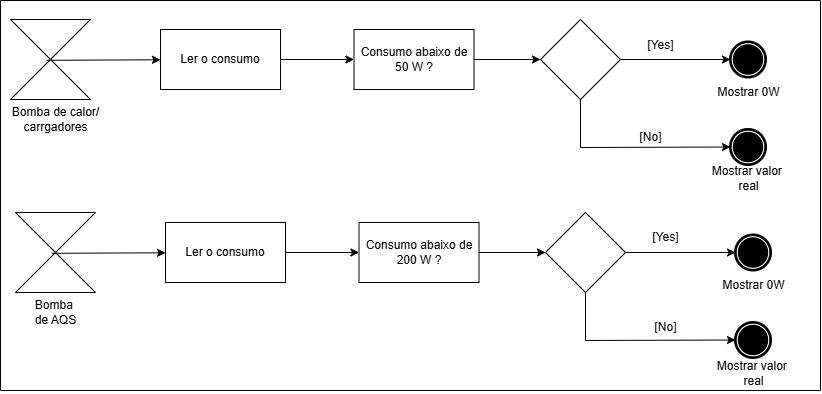
\includegraphics[width=\textwidth]{images/consumo_2.png}
    \caption{Diagrama de decisão bombas/carregadores}
    \label{fig:consumo_2.png}
\end{figure}

Encaixar todas as cards e entidades na main dashboard, foi também uma dificuldade, pois tivemos que encontrar o tamanho perfeito para cada, encaixando tudo na perfeição.
Também foi necessário criar um template sensor para somar os três valores de produção solar — \textit{PV1 Master}, \textit{PV2 Master} e \textit{PV1 Slave} — de forma a calcular a produção total proveniente dos painéis fotovoltaicos.\\
Adicionalmente, foi criado um sensor para o cálculo do consumo total da habitação, combinando a energia proveniente da produção solar, da rede elétrica (grid) e da bateria. No entanto, foram implementadas condições lógicas para garantir que apenas os fluxos de saída (exportação) do \textit{grid} e da bateria são considerados. Ou seja, se algum desses sistemas estiver a importar energia (ou seja, a consumir), esse valor é ignorado no cálculo do consumo total, garantindo uma leitura mais precisa e representativa da energia efetivamente utilizada na casa.\\
Adicionalmente, foi criado um botão de exportação energética com base num sensor personalizado (\textit{exportacao\_status}). Este sensor analisa o valor de potência da rede (\textit{sensor.rede\_power}) e, consoante o nível de exportação de energia para a rede (valores negativos), classifica a situação em quatro estados: \textit{ultra}, \textit{high}, \textit{medium} e \textit{low}.
Cada estado é representado visualmente através de um cartão interativo (\textit{custom:button-card}), com cores e ícones distintos que indicam se há excesso de produção solar, produção parcial ou dependência da rede elétrica. Esta abordagem permite ao utilizador identificar rapidamente o estado de exportação solar da habitação e tomar decisões informadas sobre o uso energético em tempo real. A Figura~\ref{fig:Saldo_Botao_Energetico_diagrama.drawio_2.png} ilustra o processo de decisão associado ao botão de exportação energética, com base nos níveis de potência exportada para a rede e respetiva codificação por cores.

\begin{figure}[H]
    \centering
    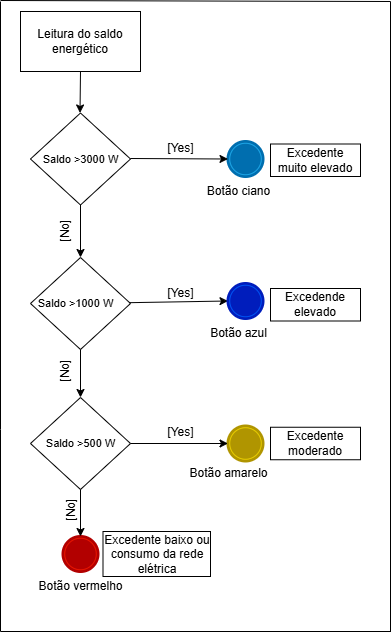
\includegraphics[height=0.4\textheight]{images/Saldo_Botao_Energetico_diagrama.drawio_2.png}
    \caption{Diagrama de decisão - Saldo energético}
    \label{fig:Saldo_Botao_Energetico_diagrama.drawio_2.png}
\end{figure}

\section{Dashboards produzidos}

\subsection{Dashboard Principal}

\begin{figure}[H]
    \centering
    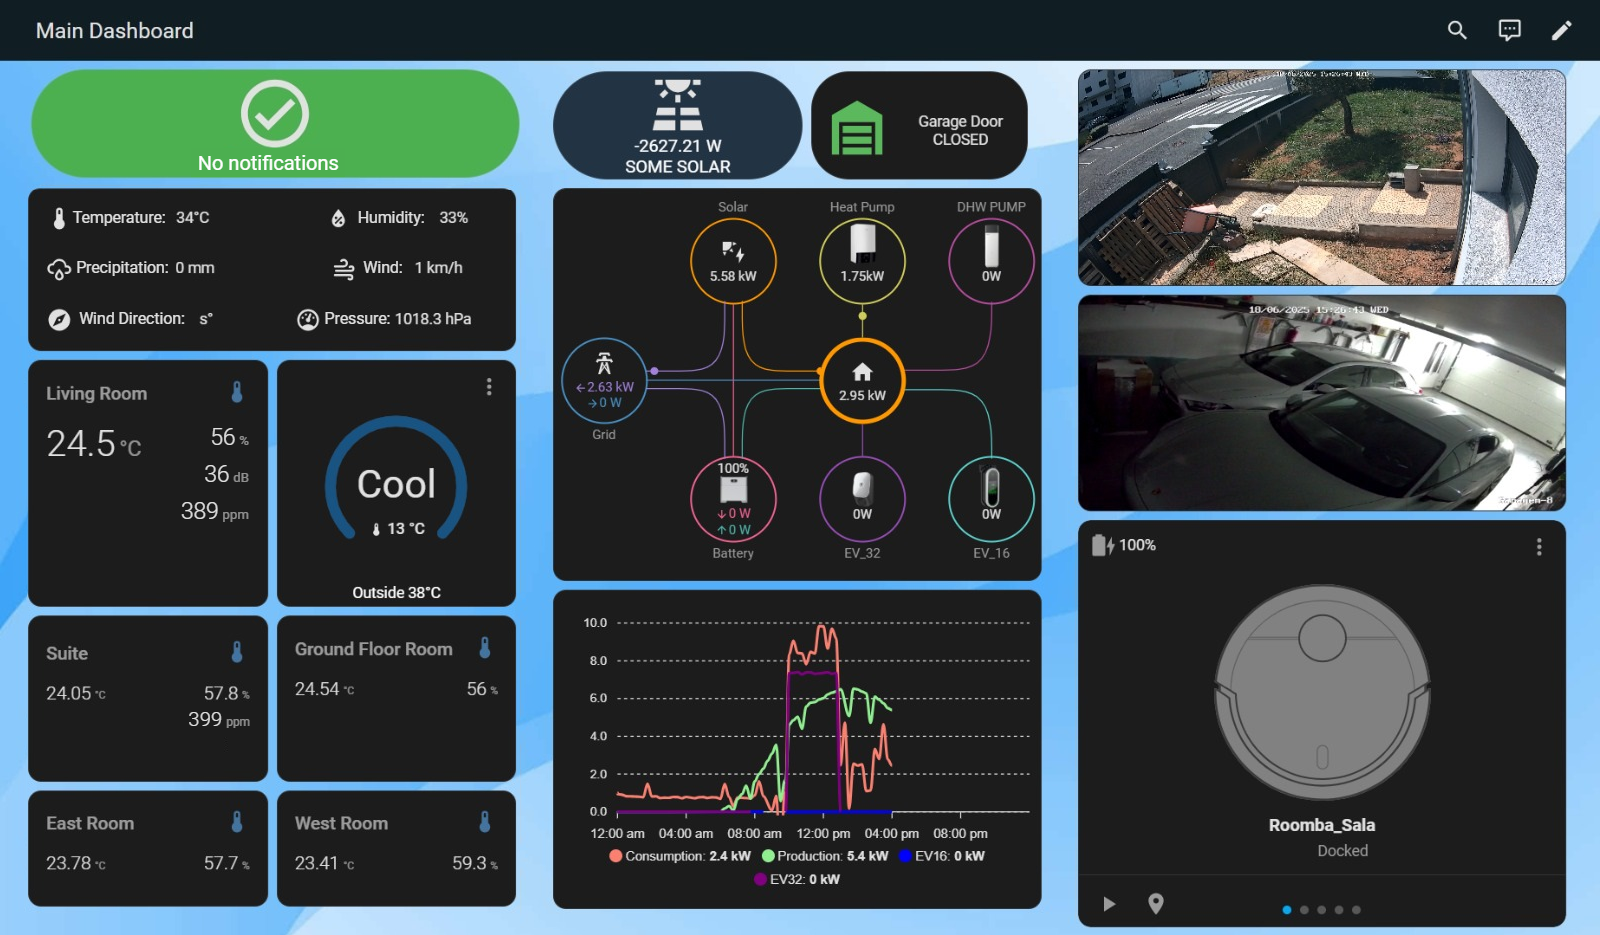
\includegraphics[width=\textwidth]{images/principal.png}
    \caption{Dashboard Principal}
    \label{fig:principal.png}
\end{figure}

A dashboard principal, chamada de \textit{Main Dashboard}, foi concebida para ser o painel principal do \gls{HA}, permitindo uma visão abrangente e imediata do estado geral da casa. Como podemos verificar na Figura~\ref{fig:principal.png}, a dashboard está dividida em três áreas distintas: a área da esquerda é dedicada ao conforto e ao ambiente, a zona central foca-se na parte energética e a área direita está orientada essencialmente à segurança. Esta organização permite uma fácil e rápida leitura da informação mais relevante da casa.

De seguida, serão explorados e explicados em detalhe os principais componentes da dashboard principal, com destaque para as integrações realizadas, os sensores utilizados, os valores apresentados em tempo real, o seu significado e as soluções adotadas para representar a informação de forma clara e funcional.




\subsubsection{Botão Notificações}

\begin{figure}[H]
    \centering
    
\includegraphics[width=0.6\textwidth]{images/botao_notificacoes.png}
    \caption{Botão Notificações}
    \label{fig:botao_notificacoes.png}
\end{figure}

O botão de notificações é uma funcionalidade essencial para garantir uma resposta rápida a eventos importantes na casa. Como ilustrado na Figura~\ref{fig:botao_notificacoes.png}, este botão assume uma aparência verde com a indicação \textnormal{"No notifications"} quando não há notificações ativas. Sempre que ocorre um evento relevante, como a abertura do portão da garagem, início de precipitação, deteção de níveis elevados de CO\textsubscript{2} (acima de 1000 ppm), ruído elevado (acima de 60 dB) ou o início de funcionamento de um robô aspirador, é gerado automaticamente um alerta visual.


\begin{table}[H]
\centering
\resizebox{!}{7.3cm}{
\rowcolors{2}{gray!10}{white}
\begin{tabularx}{\textwidth}{|p{6cm}|X|p{3cm}|}
\hline
\textbf{Condição} & \textbf{Entidade} & \textbf{Notificação} \\
\hline

Portão abriu & switch.portao\_garagem & Open gate \\

\% chuva > 0.1\%  & sensor.netatmo\_1piso\_rain\_gauge \_precipitation & Rain \\

CO2 acima de 1000  & sensor.netatmo\_1piso\_carbon \_dioxide & High CO2 \\

Noise acima de 60  & sensor.netatmo\_1piso\_noise & High Noise \\

Robo roomba da sala a limpar  & vacuum.roomba\_sala & Robot cleaning \\

Robo braava da sala a limpar  & vacuum.braava\_sala & Robot cleaning \\

Robo roomba piso a limpar  & vacuum.roomba\_piso & Robot cleaning \\

Robo roomba do bunker a limpar  & vacuum.roomba\_bunker & Robot cleaning \\

Robo roomba da cave a limpar  & vacuum.roomba\_cave & Robot cleaning \\

Bomba de calor ligou & sensor.bomba\_calor\_filtered\_power & Heat pump connected\\

Bomba de AQS ligou & sensor.bomba\_aqs\_filtered \_power & DHW pump connected\\

Vento forte & sensor.netatmo\_1piso\_anemometer \_wind\_speed &  Strong wind \\

Temperatura exterior abaixo de 0ºC & sensor.netatmo\_1piso\_netatmo \_exterior\_temperature & Negative temperature\\

Humidade exterior abaixo de 30\% & sensor.netatmo\_1piso\_netatmo \_exterior\_humidity & Negative humidity \\

Humidade exterior acima de 85\% & sensor.netatmo\_1piso\_netatmo \_exterior\_humidity & High humidity \\

Sem alertas  &  & No notifications \\

\hline
\end{tabularx}
}
\caption{Notificações, segundo condição.}
\end{table}

\subsubsection{Sensores Exteriores}

\begin{figure}[H]
    \centering
    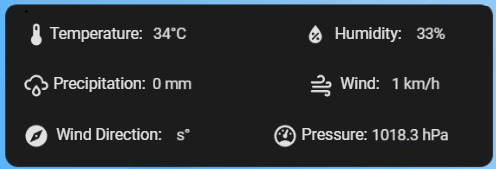
\includegraphics[width=0.6\textwidth]{images/sensores_exteriores.png}
    \caption{Sensores Exteriores}
    \label{fig:sensores_exteriores.png}
\end{figure}

A secção dos sensores exteriores (Figura~\ref{fig:sensores_exteriores.png}) fornece informação ambiental proveniente de sensores instalados no exterior da habitação. Os dados visíveis na dashboard incluem:

\begin{table}[H]
\centering
\begin{tabular}{|l|c|}
\hline
\textbf{Parâmetro}             & \textbf{Valor}       \\
\hline
Temperatura                   & 34 ºC                \\
Humidade                      & 33 \%                \\
Precipitação                  & 0 mm                 \\
Velocidade do vento           & 1 km/h               \\
Direção do vento              & Sul (S)              \\
Pressão atmosférica           & 1018.3 hPa           \\
\hline
\end{tabular}
\caption{Informações dos sensores exteriores.}
\end{table}

Estas informações são cruciais tanto para conforto como para automações, por exemplo, ajustar a climatização ou fechar estores em caso de aumento de temperatura ou vento forte.

\newpage

\subsubsection{Sensores Interiores}

\begin{figure}[H]
    \centering
    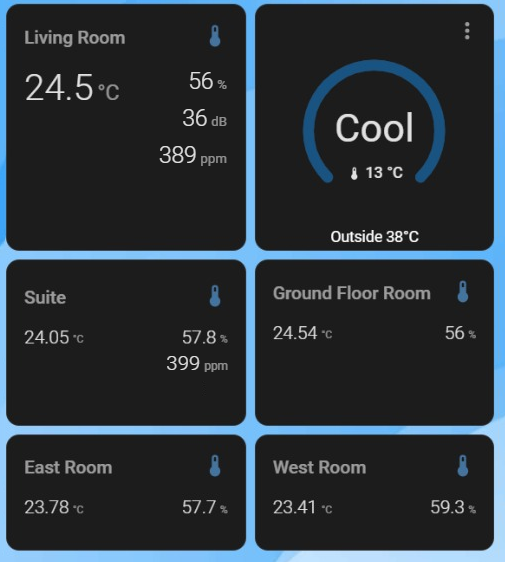
\includegraphics[width=0.6\textwidth]{images/sensores_interiores.png}
    \caption{Sensores Interiores}
    \label{fig:sensores_interiores.png}
\end{figure}

Os sensores interiores da Figura~\ref{fig:sensores_interiores.png} monitorizam temperatura, humidade, ruído e concentração de CO\textsubscript{2} em diferentes divisões da casa. Os dados disponíveis são os seguintes:

\begin{table}[H]
\centering
\begin{tabular}{|l|c|c|c|c|}
\hline
\textbf{Divisão} & \textbf{Temperatura} & \textbf{Humidade} & \textbf{Ruído} & \textbf{PPM} \\
\hline
Sala de Estar & 24.5 ºC & 56 \% & 36 dB & 389 ppm \\
Suite & 24.05 ºC & 57.8 \% & -- & 399 ppm \\
Quarto Rés-do-chão & 24.54 ºC & 56 \% & -- & -- \\
Quarto Este & 23.78 ºC & 57.7 \% & -- & -- \\
Quarto Oeste & 23.41 ºC & 59.3 \% & -- & -- \\
\hline
\end{tabular}
\caption{Dados dos sensores interiores por divisão}
\label{tab:sensores_interiores}
\end{table}

Na zona da sala, além da temperatura e humidade, é apresentado o estado atual do ar condicionado, indicando que está a arrefecer (\textit{Cool}) para atingir a temperatura da água definida de \textbf{13 ºC} e também a temperatura exterior de \textbf{38 ºC}.

\subsubsection{Botões Energia}

\begin{figure}[H]
    \centering
    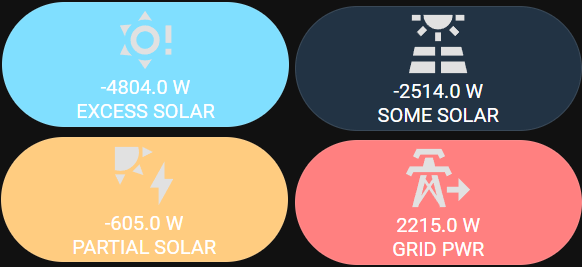
\includegraphics[width=0.6\textwidth]{botoes_energia.png}
    \caption{Botões Energia}
    \label{fig:botoes_energia.png}
\end{figure}

O botão da Figura~\ref{fig:botoes_energia.png}, fornece uma representação visual e imediata do \textbf{saldo energético} da casa, isto é, a diferença entre a energia produzida, pelos painéis solares e a consumida pela casa e seus dispositivos. A principal funcionalidade deste botão é alertar o utilizador para o estado energético com base numa escala de cores:

\begin{table}[H]
\centering
\begin{tabular}{|l|l|l|}
\hline
\textbf{Cor} & \textbf{Condição} & \textbf{Texto Botão} \\
\hline
\textcolor{cyan}{Ciano}   & Exportação superior a 3000~W & EXCESS SOLAR \\
\textcolor{blue}{Azul}    & Exportação superior a 1000~W & SOME SOLAR\\
\textcolor{yellow}{Amarelo} & Exportação superior a 500~W & PARTIAL SOLAR\\
\textcolor{red}{Vermelho} & Exportação inferior a 500~W ou consumo da rede elétrica & GRID PWR\\
\hline
\end{tabular}
\caption{Detalhe do botão de exportação de energia.}
\end{table}


\subsubsection{Botão Garagem}

\begin{figure}[H]
    \centering
    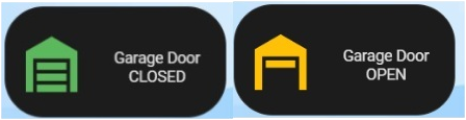
\includegraphics[width=0.6\textwidth]{botao_garagem.png}
    \caption{Botão Garagem.}
    \label{fig:botao_garagem.png}
\end{figure}

Na Figura~\ref{fig:botao_garagem.png}, temos um botão que permite controlar o \textbf{portão da garagem}, apresentando simultaneamente o seu estado atual e permitindo interagir com o sistema. A cor do botão indica o estado:

\begin{table}[H]
\centering
\begin{tabular}{|c|l|}
\hline
\textbf{Cor} & \textbf{Estado do Portão} \\
\hline
\textcolor{green}{Verde} & Portão fechado \\
\textcolor{orange}{Laranja} & Portão aberto \\
\hline
\end{tabular}
\caption{Detalhe do botão do portão.}
\label{tab:estado_portao}
\end{table}


Além da indicação visual, o botão permite também \textbf{abrir ou fechar o portão} ao ser pressionado por mais de 2 segundos, evitando assim ativações acidentais com toques breves.

\subsubsection{Diagrama Energia}

\begin{figure}[H]
    \centering
    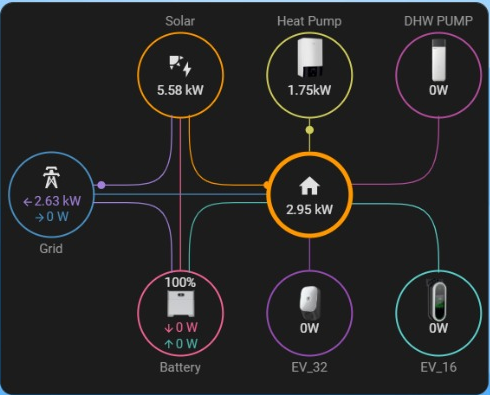
\includegraphics[width=0.6\textwidth]{images/diagrama_energia.png}
    \caption{Diagrama Energia}
    \label{fig:diagrama_energia.png}
\end{figure}

O diagrama energético apresentado na Figura.~\ref{fig:diagrama_energia.png} fornece uma representação gráfica em tempo real dos fluxos de energia entre os principais elementos do sistema energético da casa. É de fácil e rápida visualização, permitindo ao utilizador identificar rapidamente os consumos, produções e fluxos bidirecionais.

Os painéis solares encontram-se a produzir \textbf{5.58 kW}, valor superior ao consumo da habitação, que se encontra nos \textbf{2.95 kW}. A totalidade do consumo está a ser suprida pela produção solar, e o excedente de \textbf{2.63 kW} está a ser injetado na rede elétrica. A bateria encontra-se totalmente carregada (\textbf{100\%}) e, neste momento, não está nem a descarregar nem a carregar (\textbf{0 W}). Relativamente aos consumos específicos:

\begin{table}[H]
\centering
\begin{tabular}{|l|c|}
\hline
\textbf{Equipamento} & \textbf{Consumo} \\
\hline
Bomba de Calor (Heat Pump) & \textbf{1.75 kW}  \\
Bomba de Água Quente (DHW Pump) & \textbf{0 W} \\
Carregador EV\_32 & \textbf{0 W} \\
Carregador EV\_16 & \textbf{0 W} \\
\hline
\end{tabular}
\caption{Consumo dos principais equipamentos}
\label{tab:consumos_equipamentos}
\end{table}

Esta representação intuitiva permite um acompanhamento imediato do comportamento energético da habitação, facilitando ações rápidas de otimização ou diagnósticos de consumo e produção.

\subsubsection{Gráfico Energético}
\begin{figure}[H]
    \centering
    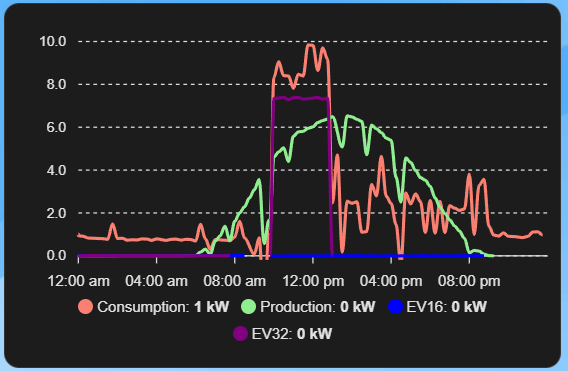
\includegraphics[width=\textwidth]{images/grafico_energia.png}
    \caption{Gráfico Energético}
    \label{fig:grafico_energia.png}
\end{figure}

O gráfico energético da Figura~\ref{fig:grafico_energia.png} apresenta a evolução do \textbf{consumo}, \textbf{produção} e utilização dos \textbf{carregadores elétricos} ao longo das últimas 24 horas. As curvas no gráfico têm as seguintes cores:

\begin{table}[H]
\centering
\begin{tabular}{|c|l|}
\hline
\textbf{Cor} & \textbf{Significado} \\
\hline
\textcolor{orange}{Laranja} & Consumo da casa \\
\textcolor{green}{Verde} & Produção fotovoltaica \\
\textcolor{violet}{Roxo} & Carregador EV\_32 \\
\textcolor{blue}{Azul} & Carregador EV\_16 \\
\hline
\end{tabular}
\caption{Detalhe do gráfico energético.}
\label{tab:cores_consumo_producao}
\end{table}

\vspace{1em}

\begin{flushleft}
\vspace{-\baselineskip} % remove espaço extra que o LaTeX pode deixar
\begin{itemize}[itemsep=0pt, parsep=0pt, partopsep=0pt, topsep=0pt, leftmargin=*]
  \item O consumo da casa apresenta picos acentuados entre as 10h00 e as 13h00, e variações moderadas no restante do dia.
  \item A produção fotovoltaica inicia-se por volta das 06h30, atinge o pico por volta do meio-dia (acima dos \textbf{6 kW}) e mantém-se estável até às 15h00, diminuindo depois gradualmente.
  \item O carregador EV\_32 esteve ativo apenas entre as 10h00 e as 14h00, coincidindo com o período de maior produção solar.
  \item O carregador EV\_16 continua sem registos de utilização significativos.
\end{itemize}
\end{flushleft}




Este gráfico permite identificar claramente os períodos de maior produção e consumo energético, contribuindo para uma gestão otimizada do autoconsumo e do carregamento de veículos elétricos com base no excedente solar disponível.

\subsubsection{Câmaras}

\begin{figure}[H]
    \centering
    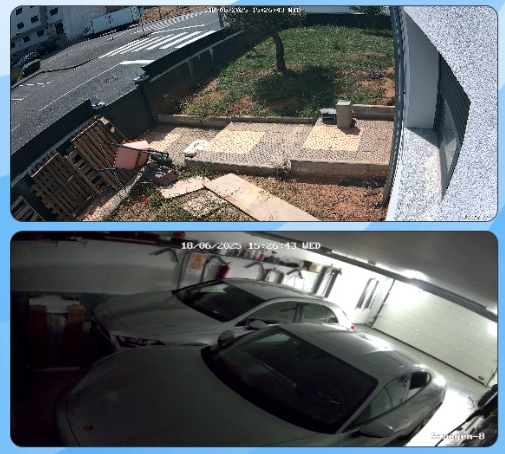
\includegraphics[width=0.6\textwidth]{images/camaras_main.png}
    \caption{Câmaras}
    \label{fig:camaras_main.png}
\end{figure}

A secção de segurança da dashboard inclui uma visualização em tempo real de duas câmaras de videovigilância, conforme mostrado na Figura~\ref{fig:camaras_main.png}. A primeira câmara está direcionada para a entrada exterior da habitação, permitindo monitorizar acessos e movimentos. A segunda câmara está posicionada na garagem, garantindo a segurança dos veículos e deteção de movimentos suspeitos. A integração destas câmaras oferece maior controlo e tranquilidade ao utilizador, permitindo uma resposta rápida em caso de atividade anómala.

\subsubsection{Aspiradores}

\begin{figure}[H]
    \centering
    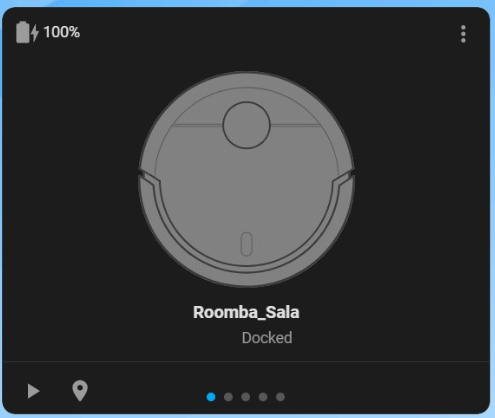
\includegraphics[width=0.6\textwidth]{images/aspiradores_main.png}
    \caption{Aspiradores}
    \label{fig:aspiradores_main.png}
\end{figure}

Na parte inferior direita da dashboard encontra-se um cartão interativo (Figura ~\ref{fig:aspiradores_main.png}) dedicado à gestão dos aspiradores robóticos. Utilizando o cartão \textit{swipe card}, é possível alternar rapidamente entre os diferentes aspiradores instalados em várias divisões da casa (5 no total). Cada cartão exibe o estado atual do dispositivo (por exemplo, “\textit{Docked}”), a bateria (por exemplo, 100\%) e permite o controlo direto de ações como iniciar ou pausar a limpeza, ou enviar o robô de volta para a base.

\newpage

\subsection{Dashboard Energia}

\begin{figure}[H]
    \centering
    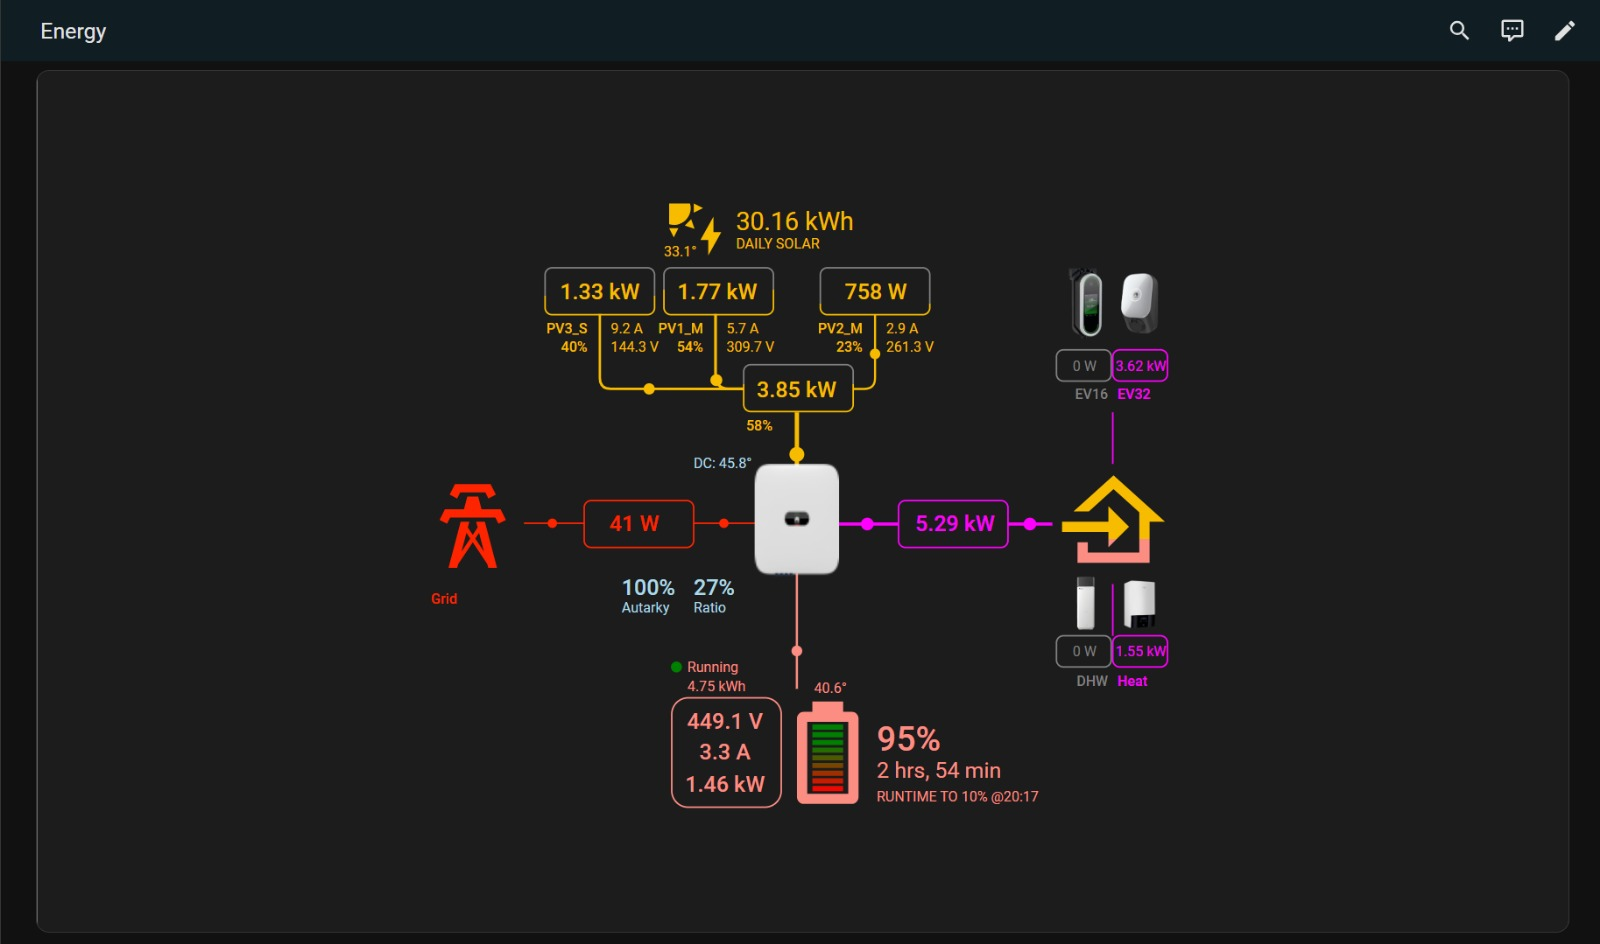
\includegraphics[width=\textwidth]{energia.png}
    \caption{Dashboard Energia}
    \label{fig:energia.png}
\end{figure}

Como mostrado na Figura.~\ref{fig:energia.png}, esta dashboard apresenta uma visão detalhada e em tempo real do sistema energético da habitação. No topo, observa-se a produção solar diária acumulada, com um total de \textbf{30,16~kWh}. Esta energia é proveniente de três \textit{strings} fotovoltaicas individuais (PV3\_S, PV1\_M e PV2\_M), que, no momento, produziam \textbf{1,33~kW}, \textbf{1,77~kW} e \textbf{758~W}, respetivamente, totalizando uma produção atual de \textbf{3,85~kW}.

Ao centro, encontra-se o inversor \textit{Huawei}, que agrega a produção solar e gere a distribuição da energia. A casa consome, neste momento, \textbf{5,29~kW}, com destaque para o carregamento do veículo \textit{EV32}, que consome \textbf{3,62~kW}, e para o sistema de aquecimento, responsável por \textbf{1,55~kW}. Os restantes dispositivos ligados à casa, nomeadamente o \textit{EV16} e o sistema de \textit{DHW} (águas quentes sanitárias), encontram-se em \textit{standby}, apresentando, por isso, um consumo de \textbf{0~W}. Este valor foi definido para simplificar a visualização da interface, considerando-se como \textit{standby} os seguintes critérios: consumos inferiores a \textbf{50~W} nos carregadores de veículos elétricos (\textit{EV}) e na bomba de \textit{AQS}, bem como consumos inferiores a \textbf{200~W} no sistema de bomba de calor. Nestes casos, o valor apresentado é \textbf{0~W}.

No lado esquerdo do diagrama, é visível a importação de energia da rede elétrica, com um valor de \textbf{41~W}. Isto indica que, apesar da produção solar, a energia gerada não é suficiente para suprir totalmente o consumo atual.

Na parte inferior, encontra-se o estado da bateria, que está com 95\% de carga e fornece \textbf{1,46~kW} para ajudar a suprir o consumo da casa. A estimativa de autonomia restante indica cerca de 2~horas e 54~minutos até atingir 10\% de carga, por volta das 20:17. A temperatura interna da bateria é de 40{,}6~ºC.

Este \textit{layout} dinâmico e intuitivo permite uma leitura clara dos fluxos energéticos entre os vários componentes: produção solar, rede elétrica, bateria, consumos da casa, consumo da bomba de calor e \textit{AQS}, e carregamento do veículo elétrico.

O uso do cartão \textit{"Picture Elements Card"} foi essencial para sobrepor ícones representativos dos dispositivos reais, tornando a visualização mais interativa e compreensível para o utilizador.

\subsection{Dashboard de aquecimento}

\begin{figure}[H]
    \centering
    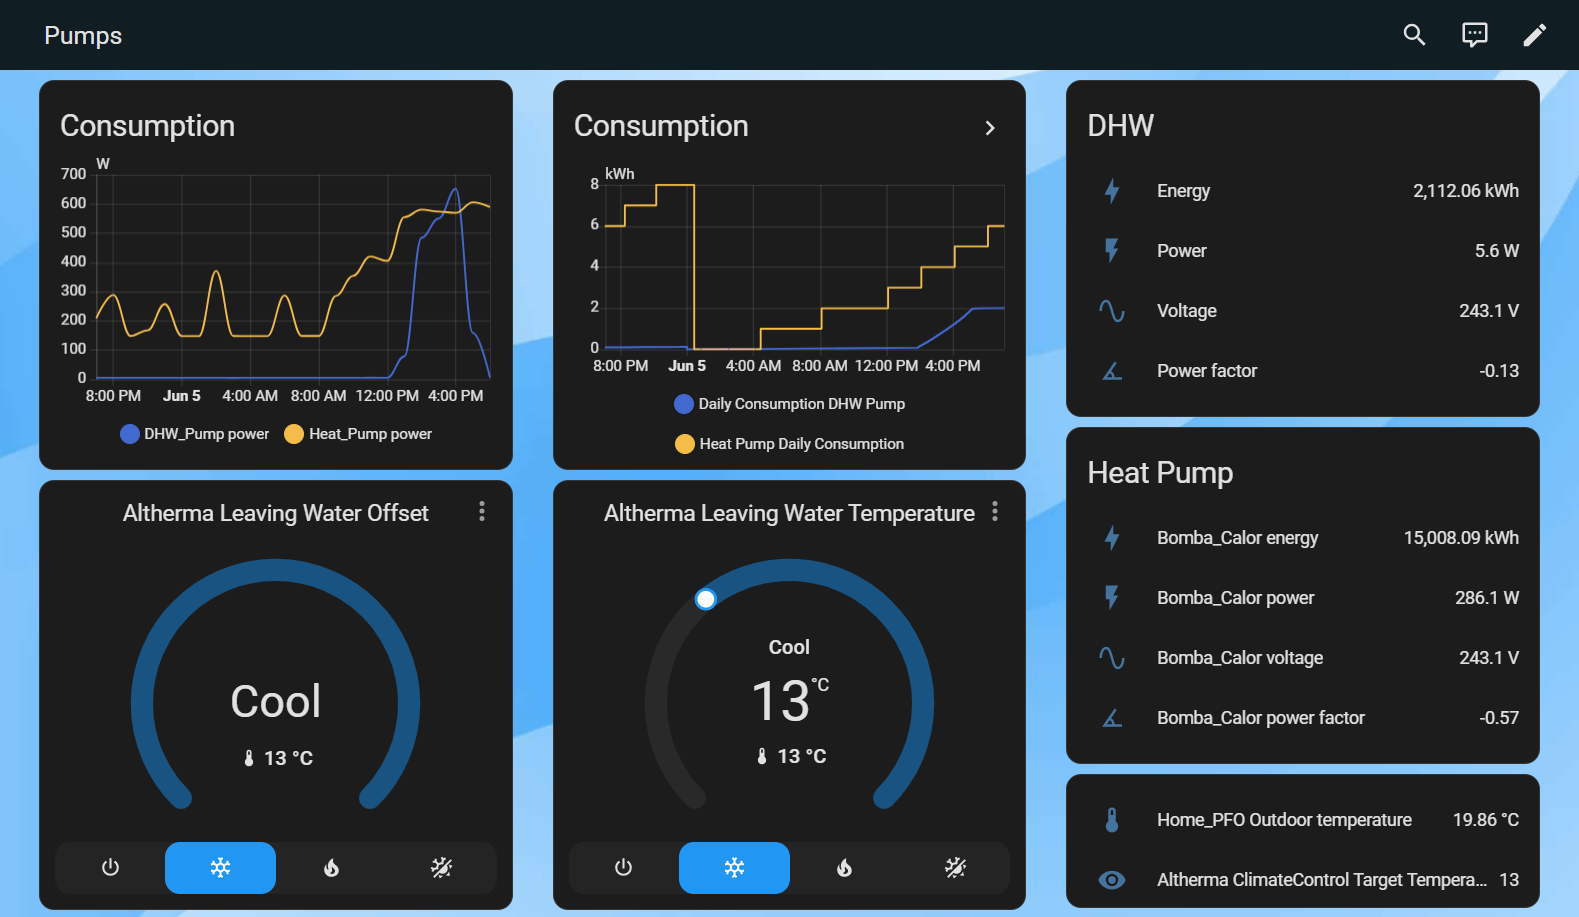
\includegraphics[width=\textwidth]{bombas.png}
    \caption{Dashboard Bombas}
    \label{fig:bombas.png}
\end{figure}

A interface apresentada na Figura~\ref{fig:bombas.png} fornece uma visão clara e organizada do sistema de aquecimento, com foco na bomba de calor \textit{Altherma} e na bomba de água quente sanitária (AQS). O dashboard está dividido em vários componentes principais:

\begin{itemize}
    \item \textbf{Gráficos de Consumo Diário e Potência}:
    \begin{itemize}
        \item \textbf{Consumo Diário da Bomba de Calor}: um gráfico complementar que reforça a análise do consumo diário de energia do sistema \textit{Altherma}.
        \item \textbf{Consumo Diário da Bomba AQS}: mostra o consumo diário da bomba de AQS, com um aumento constante ao longo do dia, ultrapassando os 8 kWh.
        \item \textbf{Potência da Bomba AQS}: mostra a potência da bomba de AQS, atingindo valores superiores a 500 W.
        \item \textbf{Potência da Bomba de Calor}: mostra a potência da bomba de calor.
    \end{itemize}
    
    \item \textbf{Controlo de Temperatura e Modo} (canto inferior esquerdo): Dois cartões de controlo permitem o ajuste direto da temperatura e do modo de funcionamento da bomba:
    \begin{itemize}
        \item \textbf{Aquecimento}: De momento desligado, OFF, e em modo \textit{Arrefecimento}, com a temperatura de saída da água definida para 13 ºC.
        \item \textbf{Arrefecimento}: também definido para 13 ºC, com o sistema a operar ativamente em modo de arrefecimento.
    \end{itemize}
    
    \item \textbf{Informações Adicionais} (direita): Apresenta métricas complementares do sistema, como o consumo de energia da bomba AQS (2110.11 kWh), potência (7.1 W), voltagem (241.6 V) e fator de potência (-0.17). Para a bomba de calor, o consumo de energia é de 15003.56 kWh, com um consumo atual de potência de 1132.9 W, voltagem de 241.6 V e fator de potência de -0.91. A temperatura exterior é de 14.41ºC, e a temperatura alvo da \textit{Altherma} está atualmente definida para 13ºC.
\end{itemize}

\newpage

\subsection{Dashboard Termostatos}

\begin{figure}[H]
    \centering
    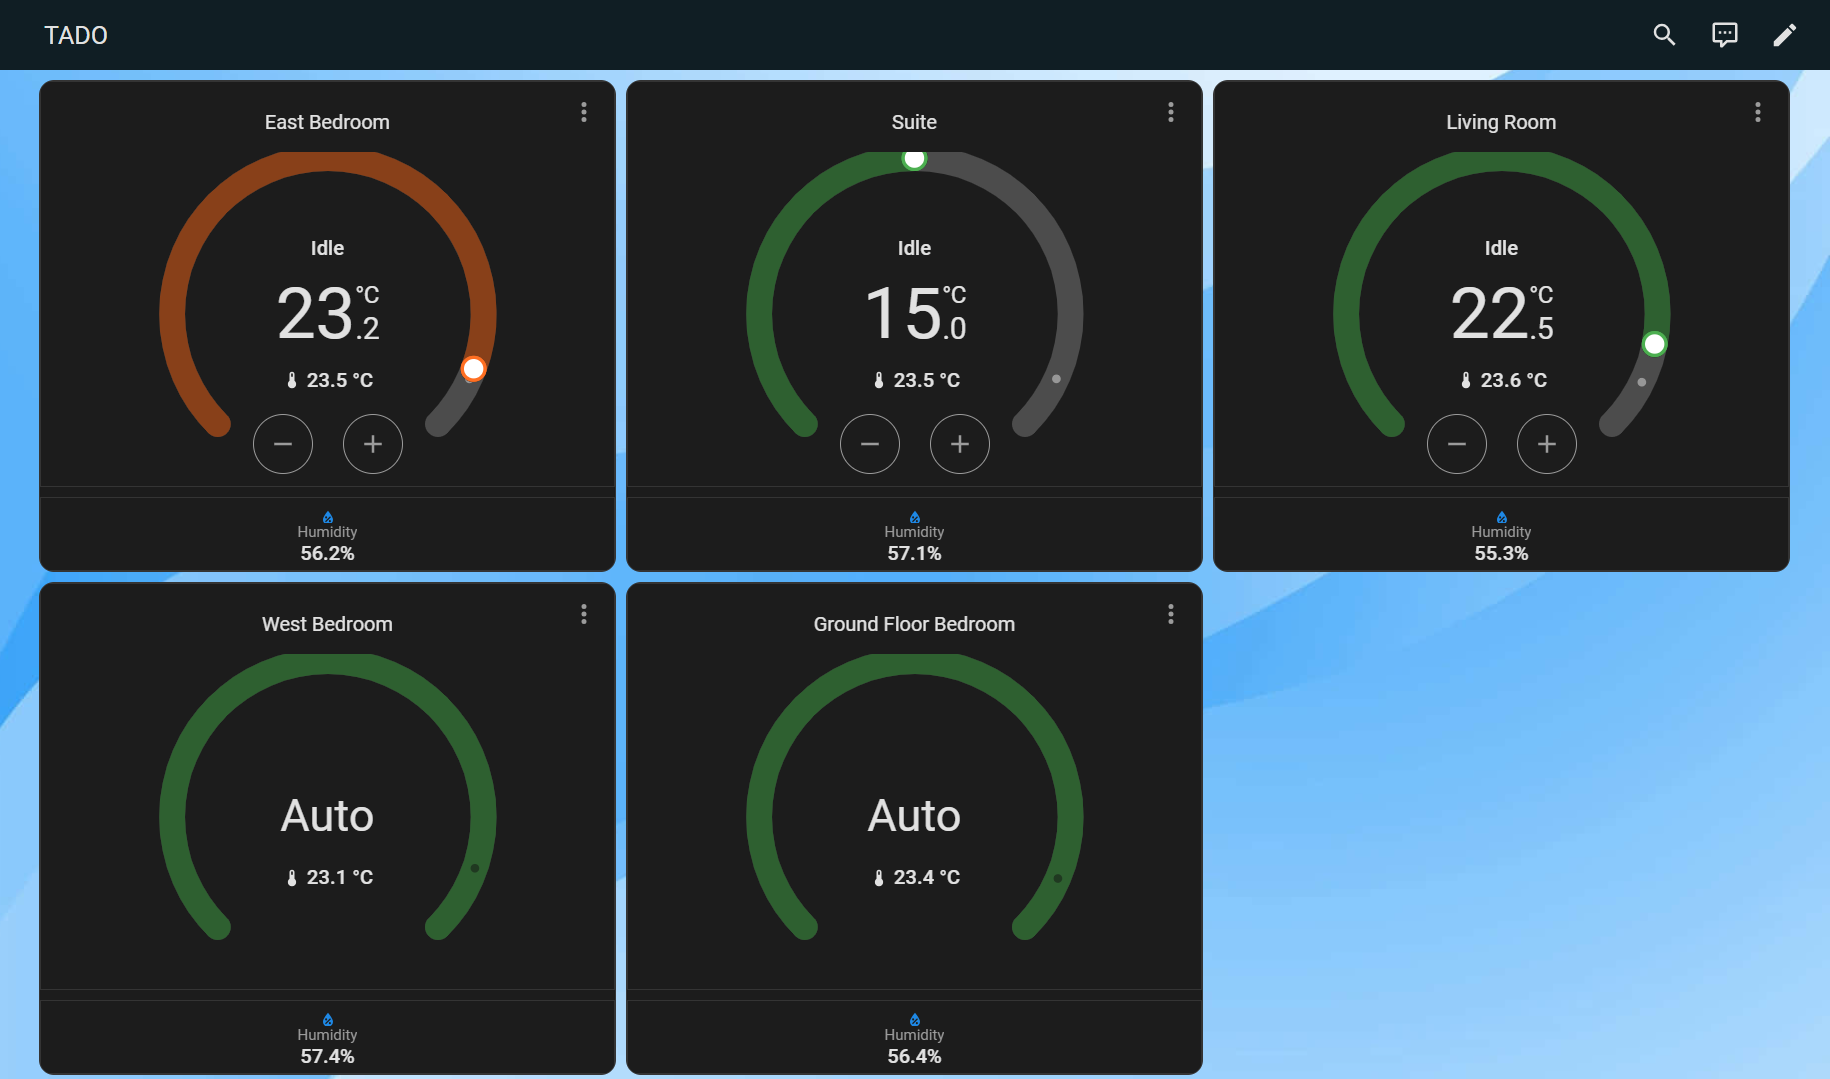
\includegraphics[width=\textwidth]{termostatos.png}
    \caption{Dashboard Termostatos}
    \label{fig:termostatos.png}
\end{figure}

A Figura~\ref{fig:termostatos.png} fornece uma visão abrangente do sistema de controlo climático interior, apresentando o estado atual dos termóstatos em várias divisões da casa. Cada cartão mostra a temperatura atual, a humidade relativa e o modo de funcionamento configurado (por exemplo, \textit{Auto} ou valor manual definido).

Segue-se um resumo dos dados apresentados:

\begin{itemize}
    \item \textbf{Quarto Este}: A temperatura atual é de 23,2ºC e o termóstato está definido manualmente para 23,1ºC. A divisão encontra-se inativa e a humidade é de 51,5\%.
    
    \item \textbf{Suite}: O termóstato está definido para uma temperatura alvo bastante inferior, 15,0ºC, enquanto a temperatura atual da divisão é de 23,4ºC, com uma humidade de 51,8\%. Isto sugere que está previsto arrefecimento, mas o sistema permanece inativo.
    
    \item \textbf{Sala de Estar}: A temperatura alvo é de 22,5ºC, com uma temperatura real de 23,6ºC e 50,1\% de humidade. O sistema encontra-se inativo, o que é expectável devido à pequena diferença entre a temperatura atual e a desejada.
\end{itemize}

Esta interface proporciona tanto visibilidade em tempo real como controlo sobre as condições térmicas de cada área da habitação. Promove a eficiência energética ao permitir ao utilizador adaptar o sistema de climatização apenas onde é necessário, e identificar divisões com temperaturas ou níveis de humidade inconsistentes.


\subsection{Dashboard Vigilância}

\begin{figure}[H]
    \centering
    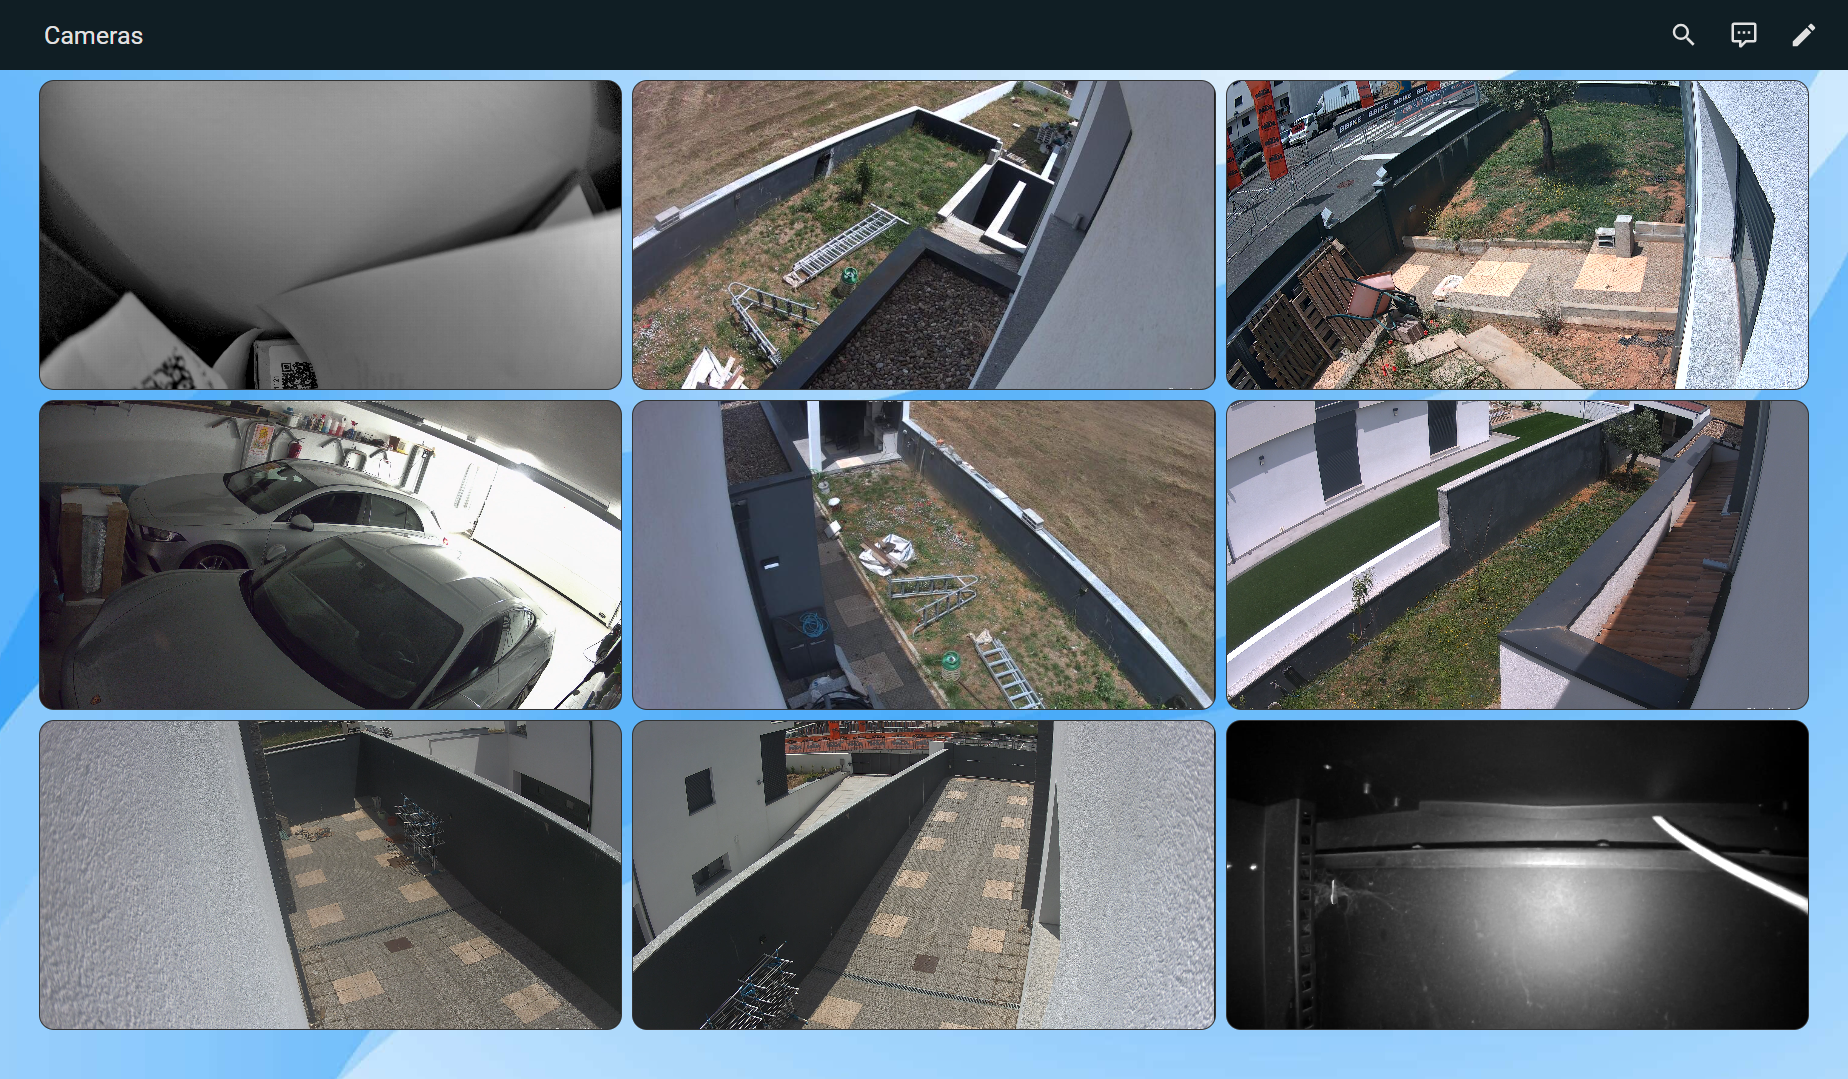
\includegraphics[width=\textwidth]{camaras.png}
    \caption{Dashboard Vigilância}
    \label{fig:camaras.png}
\end{figure}


Como mostrado na Figura~\ref{fig:camaras.png}, esta dashboard é inteiramente dedicada à monitorização em tempo real do sistema de videovigilância da propriedade. Apresenta uma grelha estruturada com nove transmissões de câmaras, cobrindo várias áreas exteriores. As câmaras captam diferentes perspetivas dos arredores, incluindo caminhos de acesso, paredes laterais e zonas do perímetro.

A imagem central na segunda linha mostra claramente o interior da garagem. É de notar que a transmissão da câmara no canto inferior direito corresponde a uma integração com a Netatmo, que fornece cobertura adicional com capacidades de deteção inteligente.

\subsection{Dashboard Estores}

\begin{figure}[H]
    \centering
    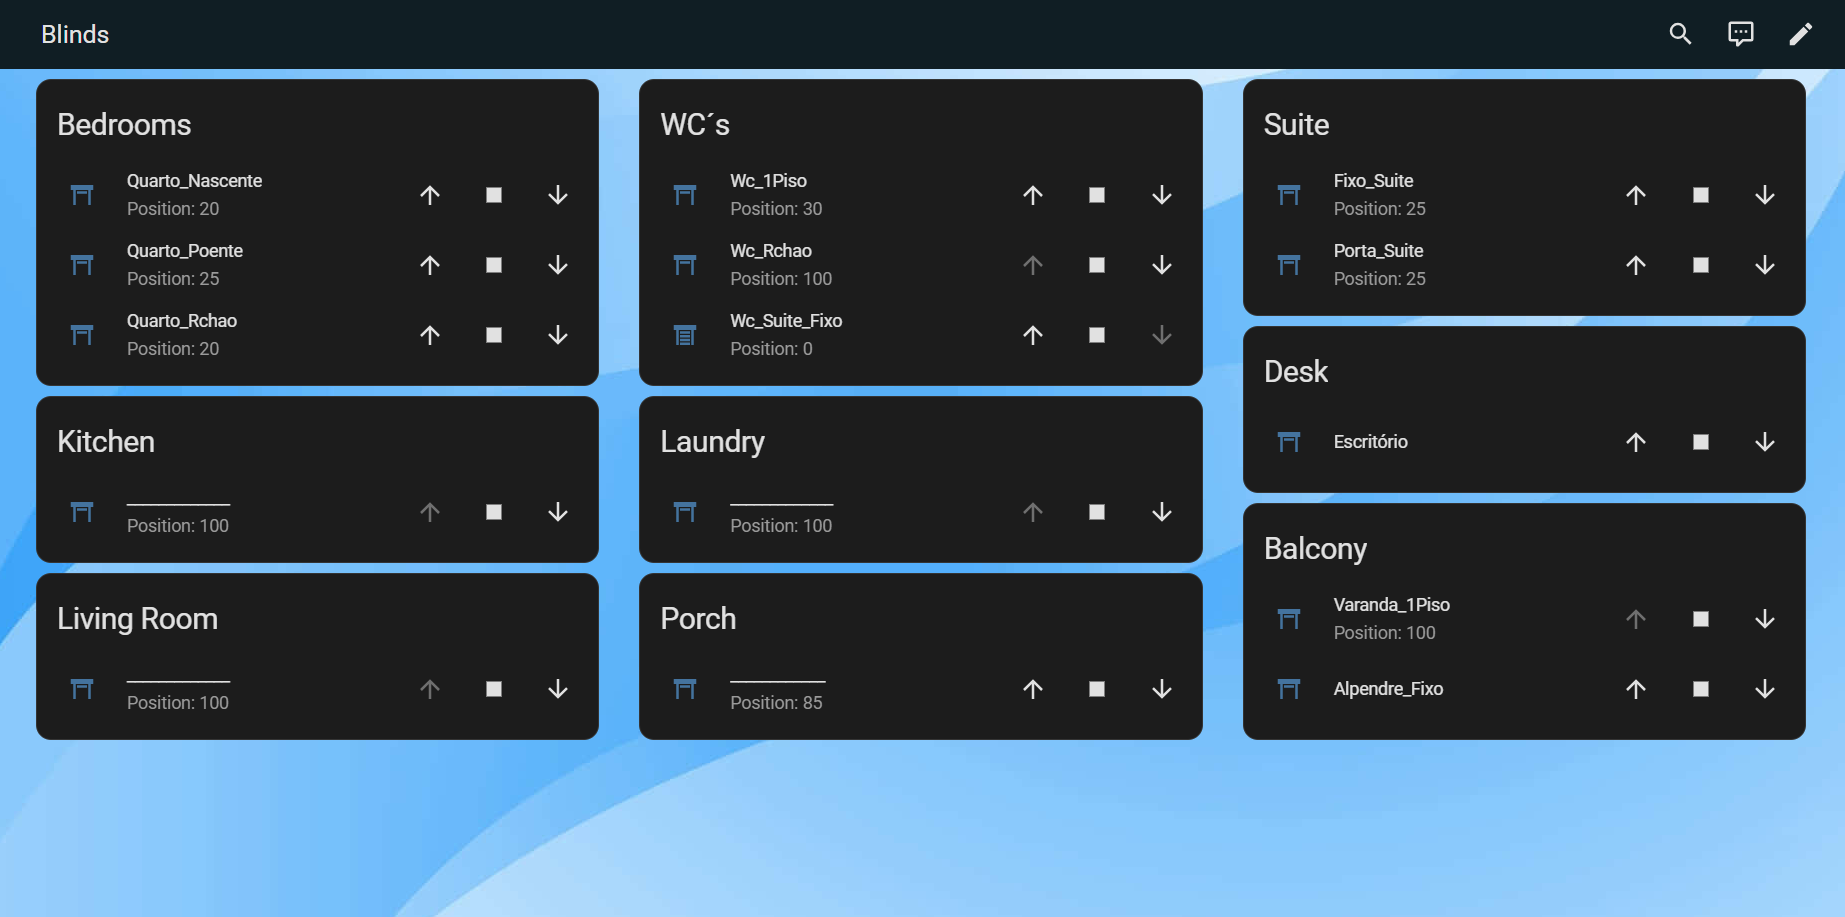
\includegraphics[width=\textwidth]{images/estores.png}
    \caption{Dashboard Estores}
    \label{fig: estores.png}
\end{figure}

Na Figura~\ref{fig: estores.png} é possível observar a dashboard dos estores com 3 botões cada:

\begin{itemize}
    \item \textbf{Seta para cima}: abre o estore.
    \item \textbf{Botão quadrado}: pára o estore na posição atual.
    \item \textbf{Seta para baixo}: fecha o estore.
\end{itemize}

As divisões com múltiplos estores (como a \textit{Suite} ou os \textit{Quartos}) apresentam cada dispositivo individualmente com o respetivo nome. O layout é responsivo e foi desenhado para permitir uma identificação visual rápida e controlo manual de todos os estores automatizados da habitação.

É ainda possível observar a sua posição, sendo "100\%" aberto e "0\%" fechado.

\newpage


\subsection{Dashboard Informação Ambiental}

\begin{figure}[H]
    \centering
    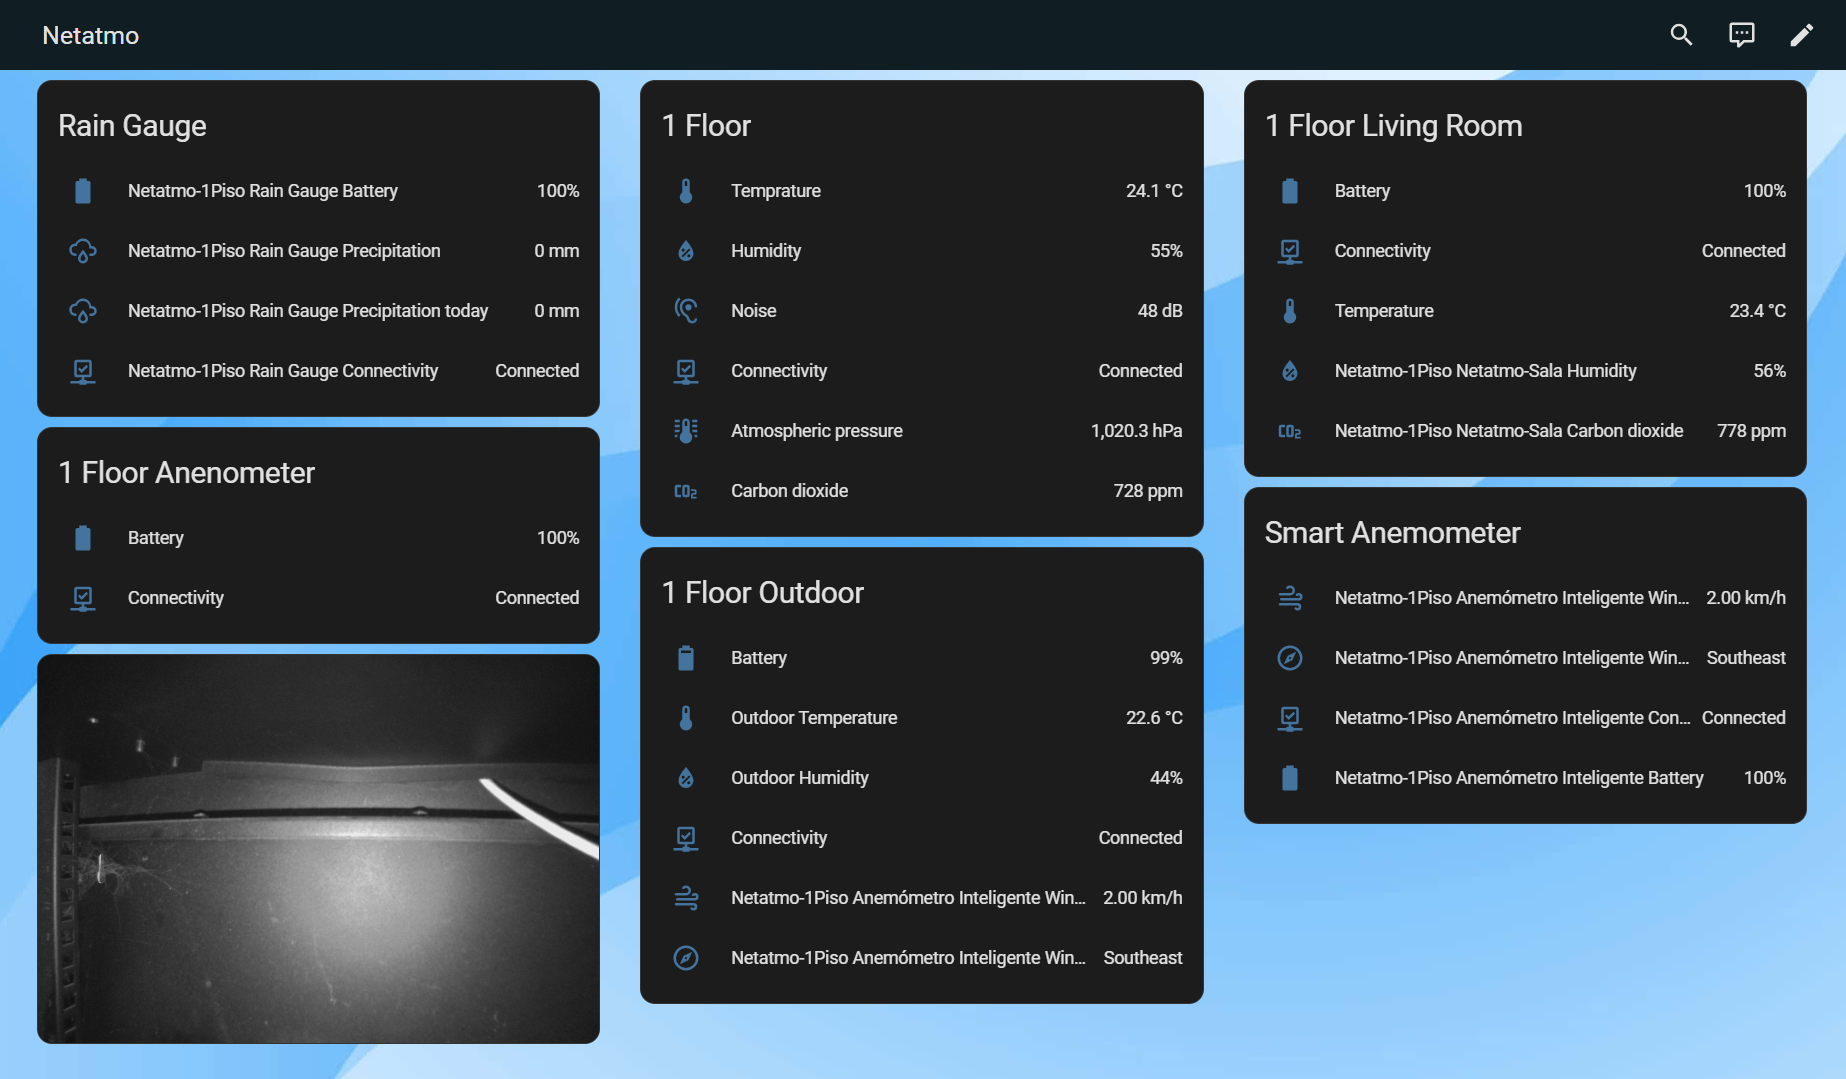
\includegraphics[width=\textwidth]{images/netatmo.png}
    \caption{Dashboard Informação Ambiental}
    \label{fig: netatmo.png}
\end{figure}

A Figura~\ref{fig: netatmo.png} apresenta o dashboard da informação ambiental, que fornece uma visão compacta e clara de vários sensores distribuídos pela casa. No canto inferior esquerdo, uma transmissão de câmara monitoriza a área física onde estão instalados alguns dos sensores.

O cartão \textnormal"1 Floor" (centro superior) exibe o módulo interior principal, localizado no primeiro andar, com leituras de temperatura (24,1ºC), humidade (55\%), ruído (48 dB), pressão atmosférica (1020,3 hPa) e CO2 (728 ppm), com conectividade ativa.

Na secção “1 Floor Living Room”, o módulo apresenta uma temperatura de 23,4ºC, humidade de 56\% e concentração de CO2 de 778 ppm, também com ligação estável. O módulo exterior, indicado em “1 Floor Outdoor”, reporta uma temperatura de 22,6ºC e humidade de 44\%, com bateria a 99\% e conectividade ativa.

O módulo “Rain Gauge” regista precipitação atual e diária como 0 mm, com ligação estável e bateria a 100\%. Já o módulo "Smart Anemometer" regista a velocidade do vento.

Este dashboard proporciona um acesso centralizado a dados meteorológicos e à qualidade do ar interior, permitindo melhor controlo e gestão ambiental no contexto da casa inteligente.


\subsection{Dashboard Robos-Aspirador}

\begin{figure}[H]
    \centering
    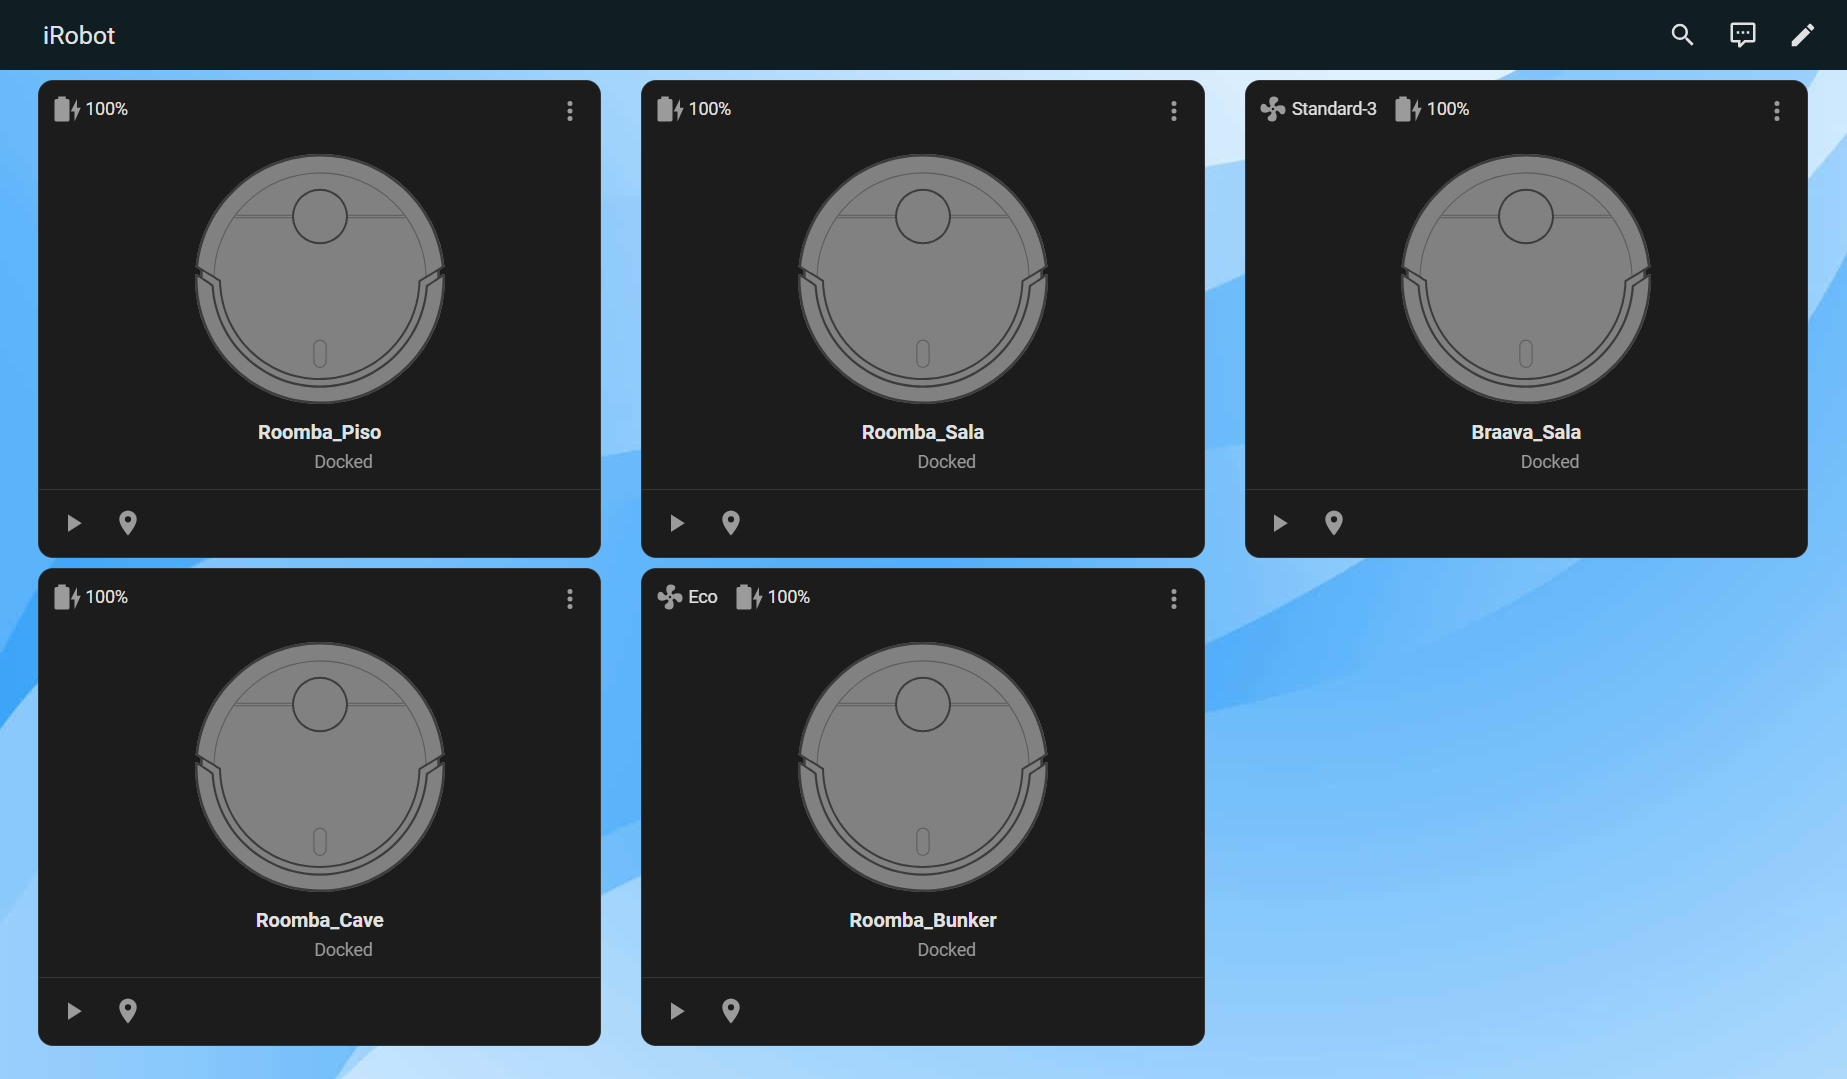
\includegraphics[width=\textwidth]{images/irobot.png}
    \caption{Dashboard Robos-Aspirador}
    \label{fig: irobot.png}
\end{figure}

A Figura~\ref{fig: irobot.png} apresenta uma dashboard do \gls{HA} dedicada à integração com dispositivos robos aspiradores. Cada cartão da dashboard representa um robô aspirador individual, com indicação clara do seu nome, estado, nível de bateria e modo de funcionamento. Os dispositivos mostrados incluem: Roomba\_Piso, Roomba\_Sala, Braava\_Sala, Roomba\_Cave e Roomba\_Bunker. Todos os aspiradores encontram-se atualmente no estado "Docked", ou seja, estacionados nas respetivas bases de carregamento, com a bateria completamente carregada (100\%). O cartão utilizado foi o "Vacuum Card", instalado a partir do \gls{HACS}.\\

\section{Integração com Alexa}

Para além das dashboards desenvolvidas, foi também implementada uma funcionalidade que permite controlar dispositivos do \gls{HA} através de comandos de voz com a assistente virtual Alexa.

A integração foi realizada de forma simples, recorrendo ao componente \textit{emulated\_hue}, que simula uma ponte \textit{Philips Hue} na rede, permitindo que a Alexa detete dispositivos expostos pelo HA. Para isso, é necessário definir o endereço IP do HA na rede local, especificar as entidades a controlar e atribuir nomes reconhecíveis por voz.

\lstset{inputencoding=ascii}
\begin{lstlisting}[language=YAML, caption={configuration.yaml}]
emulated_hue:
  type: alexa
  host_ip: ****.****.****.****  # IP da Alexa na rede local
  listen_port: 80
  expose_by_default: false
  entities:
    switch.portao_garagem:
      name: Portao
      hidden: false
\end{lstlisting}

Após inserir a configuração no ficheiro \textit{configuration.yaml} do \gls{HA}, é necessário reiniciar o sistema para aplicar as alterações. Depois do reinício, basta pedir à Alexa que procure novos dispositivos. A assistente irá detetar automaticamente o dispositivo configurado, neste caso com o nome "Portão".

Com esta configuração, ao dizer “Alexa, liga Portão” ou “Alexa, abre Portão”, a assistente interpreta o comando de voz e envia a instrução correspondente ao \gls{HA}. O ideal será utilizar o primeiro comando, uma vez que o portão da garagem está configurado como um interruptor (switch) que alterna entre os estados ligado e desligado. O \gls{HA}, ao receber o comando, ativa a entidade \textit{switch.portao\_garagem}, o que resulta na abertura do portão. Esta integração permite um controlo por voz prático, eficiente e totalmente local, sem necessidade de dependência da cloud ou de configurações adicionais externas.

Para ler estados de sensores, como por exemplo a temperatura da sala, a solução foi um pouco mais complexa. O \textit{emulated\_hue} reconhece apenas dispositivos que se comportem como interruptores, luzes, ou scripts, ou seja, não consegue ler diretamente sensores como \textit{sensor.termometro\_sala\_temperatura}.\\
Por isso, para conseguir que a Alexa "leia" a temperatura da sala, foi necessário contornar esta limitação com a seguinte abordagem:\\

Em primeiro lugar, foi criado um \textit{input\_boolean} chamado \textit{temperatura\_sala}, que simula um interruptor virtual. Este interruptor foi exposto à Alexa através do \textit{emulated\_hue}, com o nome “sala”. Assim, ao dizer “Alexa, liga sala”, ou simplesmente “Alexa, sala”,  a Alexa aciona esse interruptor, como se estivesse a ligar uma lâmpada:

\newpage

\lstset{inputencoding=ascii}
\begin{lstlisting}[language=YAML, caption={configuration.yaml}]
emulated_hue:
  type: alexa
  host_ip: ****.****.****.****  # IP da Alexa na rede local
  listen_port: 80
  expose_by_default: false
  entities:
    input_boolean.temperatura_sala:
      name: sala
      hidden: false

input_boolean:
  temperatura_sala:
    name: Perguntar temperatura
    initial: off
\end{lstlisting}

De seguida, foi criado um script no \gls{HA} que envia uma mensagem de texto-para-fala (TTS) para a Alexa com a leitura atual da temperatura. Este script utiliza a integração \textit{Alexa Media Player}, recorrendo à entidade \textit{notify.alexa\_media\_<dispositivo>} para falar diretamente através do dispositivo Alexa, utilizando a seguinte lógica:

\lstset{inputencoding=ascii}
\begin{lstlisting}[language=YAML, caption={configuration.yaml}]
sequence:
  - action: notify.alexa_media_*nome_do_dispositivo*
    data:
      message: >-
        A temperatura atual da sala e de {{
        states('sensor.netatmo_1piso_netatmo_sala_temperature') 
        }} graus.
      data:
        type: tts
alias: Alexa
description: ""
\end{lstlisting}

\vspace{-180pt}

\newpage

Por fim, foi criada uma automatização que tem como gatilho o momento em que o \textit{input\_boo-lean.temperatura\_sala} muda para o estado “on”. Quando isso acontece, a automação executa automaticamente o script anteriormente definido, fazendo com que a Alexa diga a temperatura da sala ao utilizador.

Para que o sistema funcione de forma contínua e não fique bloqueado após uma primeira utilização, a automação também inclui uma ação adicional que desliga o \textit{input\_boolean} alguns segundos depois de ser ativado. Este passo garante que a automação possa ser novamente acionada no futuro com o mesmo comando de voz.

\lstset{inputencoding=ascii}
\begin{lstlisting}[language=YAML, caption={configuration.yaml}]
alias: Alexa
description: ""
trigger:
  - platform: state
    entity_id:
      - input_boolean.temperatura_sala
    from: "off"
    to: "on"
condition: []
action:
  - service: script.alexa
    data: {}
  - service: input_boolean.turn_off
    target:
      entity_id: input_boolean.temperatura_sala
mode: single

\end{lstlisting} 

Esta abordagem permite contornar a limitação do \textit{emulated\_hue}, que não reconhece sensores, utilizando entidades compatíveis (como \textit{input\_boolean}) para simular ações compreendidas pela Alexa. Combinando um \textit{input\_boolean}, um script com TTS e uma automatização simples, é possível transformar comandos de voz em respostas inteligentes com dados em tempo real, como a leitura de temperatura, reforçando a integração entre o \gls{HA} e assistentes de voz.

\begin{table}[H]
\centering
\rowcolors{2}{gray!10}{white}
\begin{tabularx}{\textwidth}{|X|X|X|}
\hline
\textbf{Função} & \textbf{Comando} & \textbf{Entidade} \\
\hline

Abrir portão da garagem & "Alexa, liga Portão" & switch.portao\_garagem \\

Fechar portão da garagem & "Alexa, desliga Portão" & switch.portao\_garagem \\

Ler temperatura da sala & \textnormal"Alexa, sala" ou \textnormal"Alexa, liga sala" & sensor.netatmo\_1piso\_netat-mo\_sala\_temperature \\

\hline
\end{tabularx}
\caption{Funções, comandos e entidades associadas na integração da Alexa}
\end{table}